\documentclass[tikz,border=5pt]{standalone}
\usepackage[T1]{fontenc}
\usepackage{lmodern}
\usepackage{pgfplots}
\pgfplotsset{compat=1.18}
\definecolor{holdc}{RGB}{76,120,168}
\definecolor{ordc}{RGB}{209,143,0}
\definecolor{sapgray}{RGB}{122,122,122}
\definecolor{llmred}{RGB}{190,60,50}
\definecolor{runtwo}{RGB}{38,108,165}
\definecolor{greenc}{RGB}{70,140,90}
\begin{document}
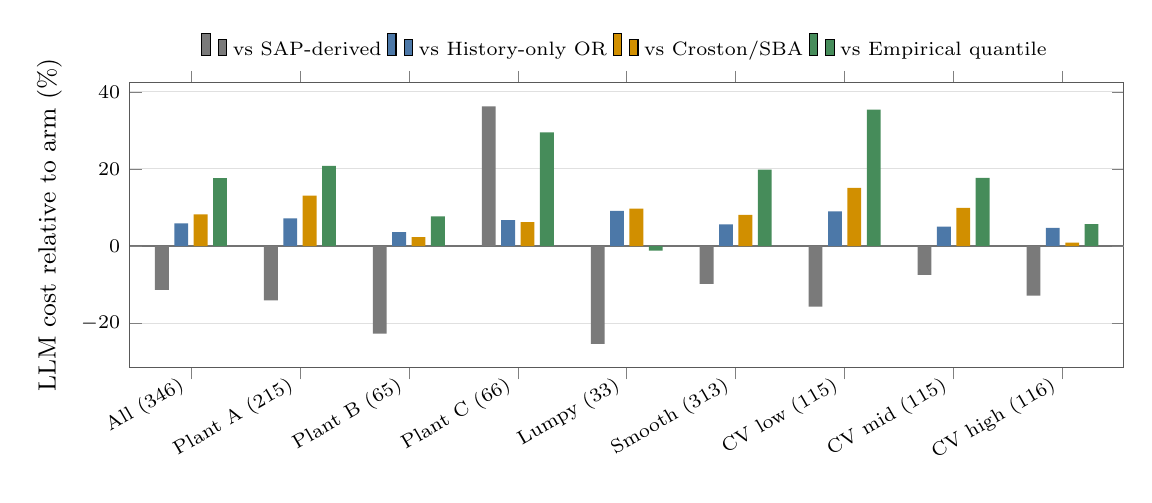
\begin{tikzpicture}
\begin{axis}[
  width=14.2cm,height=5.2cm,
  ybar,bar width=5pt,
  symbolic x coords={all,a,b,c,lumpy,smooth,cvl,cvm,cvh},xtick=data,xticklabels={{All (346)},{Plant A (215)},{Plant B (65)},{Plant C (66)},{Lumpy (33)},{Smooth (313)},{CV low (115)},{CV mid (115)},{CV high (116)}},
  xticklabel style={font=\scriptsize,rotate=30,anchor=east},
  yticklabel style={font=\scriptsize},
  ylabel={LLM cost relative to arm (\%)},ylabel style={font=\small},
  ymajorgrids=true,grid style={black!12},axis line style={black!65},
  extra y ticks=0,extra y tick style={grid=major,grid style={black!55}},extra y tick labels={},
  enlarge x limits=0.07,
  legend style={font=\scriptsize,at={(0.5,1.04)},anchor=south,draw=none,fill=none},legend columns=4,
]
  \addplot[fill=sapgray,draw=none] coordinates {(all,-11.4) (a,-14.1) (b,-22.7) (c,36.2) (lumpy,-25.4) (smooth,-9.8) (cvl,-15.7) (cvm,-7.5) (cvh,-12.9)};
  \addplot[fill=holdc,draw=none] coordinates {(all,5.9) (a,7.2) (b,3.6) (c,6.7) (lumpy,9.1) (smooth,5.6) (cvl,9.0) (cvm,5.0) (cvh,4.7)};
  \addplot[fill=ordc,draw=none] coordinates {(all,8.2) (a,13.1) (b,2.3) (c,6.2) (lumpy,9.7) (smooth,8.1) (cvl,15.1) (cvm,9.9) (cvh,0.9)};
  \addplot[fill=greenc,draw=none] coordinates {(all,17.6) (a,20.8) (b,7.7) (c,29.5) (lumpy,-1.2) (smooth,19.8) (cvl,35.4) (cvm,17.7) (cvh,5.7)};
  \legend{vs SAP-derived,vs History-only OR,vs Croston/SBA,vs Empirical quantile}
\end{axis}
\end{tikzpicture}
\end{document}
